\section{Real World application}

A general s-plex application that is probably used is the identification of group or friend networks
where one can make assumptions about group or friend networks. This is application is not directly
derived from our programming assignment, but it is somewhat related since one still has to identify k-plexes in a
undirected graph which with the amount of people using social media these days is not trivial.
An application that is closer to the given s-plex programming assignment would be telecommunication networks.
Where the distance between the antennas, towers or compute node could be correlated to the weight matrix and the s-plex
relaxation of the clique's could be used to make crucial system more reduntant (low s-plexes) and other less crucial systems
less reduntant (higher s-plexes).

\section{Deterministic Construction Heuristic}

Our first idea for a construction of solutions is the following: An empty graph (without edges) is always 
a 1-plex, since a single node without edges is a 1-plex. Removing all the edges gives a valid solution, 
however a very bad one. Our first idea for an algorithm that finds a good solution was to start with an 
empty graph and go through all the edges in $A_0$, check if adding them to $A$ is legal and if so, do that. 
This algorithm improves the empty graph, however it can only find $s$-plexes of up to $|S|=s+1$. The reason 
is that it will connect the first node $v_1$ with $\min(s,\deg_{A_0} (v_1))$ many other nodes, then the 
cluster of $v_1$ is an $s$-plex with size at most $s+1$ and no more nodes can be added. Then, all the other 
nodes in the cluster might get connected among each other, but the $s$-plex will not get any bigger. 
Practically speaking, with this construction we got approximately $n/(s+1)$ many clusters of size $s+1$ 
which were mostly fully connected, so this construction results in small clusters.\\

\textcolor{red}{
deterministic construction heuristic where we explain how the construction heuristic is done.
Maybe only do on the problem with 9 vertices and plot some results.}

\pagebreak

\section{Randomized Construction Heuristic}

For our random construction we randomly parse the entries of $A_0$ but do the same as above otherwise.

\subsection{Local improvement move operators}
After this point we found it difficult to think of the next move, because simply adding one edge in this state 
will always yield an illegal solution. In trying to understand the problem better, we wrote the adjacency 
matrices $A_0$ in files and looked at their structure. What we found was that there is a structure in most of the 
graphs, more precisely there are 3 types of graphs (see also figure \ref{fig:types}):

\begin{enumerate}
    \item locally strongly connected: 26/60 (Here, nodes that are close in numbering are also strongly connected 
    in the graph)
    \item seemingly randomly connected: 23/60
    \item tentacle-like connected: 7/60 (Here, the Graphs have a semi-large, strongly 
    connected cluster with "tentacles" reaching out. Tentacle-shaped clusters are bad for $s$-plexes, 
    so we will have to seperate these "lines" into small "spheres".)
\end{enumerate}

\begin{figure}[h]
\centering
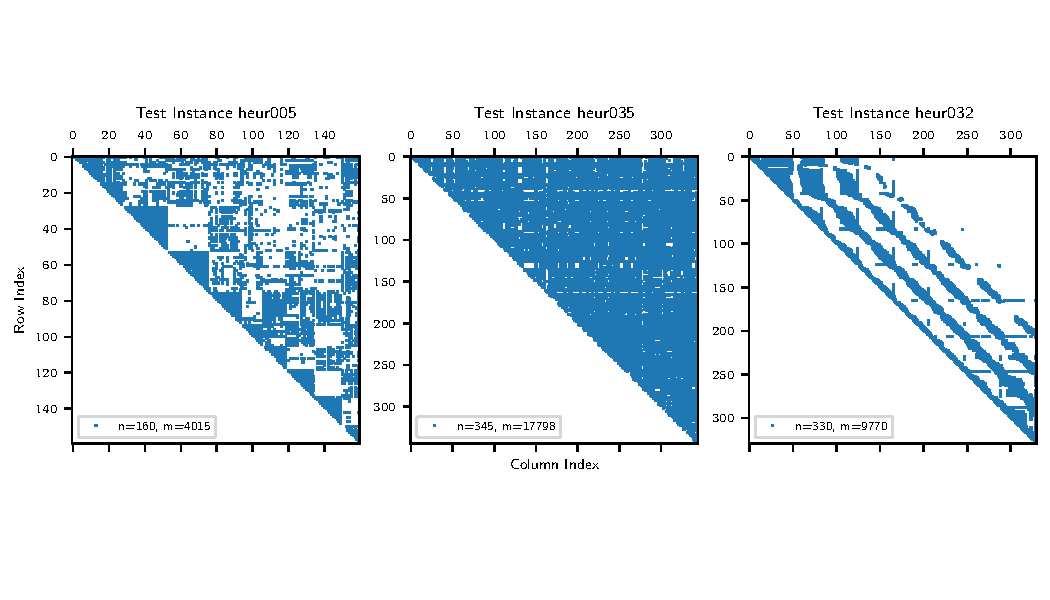
\includegraphics[width=\linewidth, trim= {0 1.8cm 0 1.8cm}, clip]{figures/spy_adjacency.pdf}
\caption{\label{fig:types}Instances of the different graph types. Left is a locally strongly 
connected graph, this is part of instance 005. In the middle is a seemingly randomly connected graph, 
which is part of instance 035. On the right is a tentacle-like connected graph, which is part of instance 032.}
\end{figure}

We will use this special structure of some instances to derive parts of our algorithms. Some might consider 
this cheating, but we think, that finding patterns in the instances is an important part of solving problems 
in real world applications so we find it to be okay. We will see later, that for the locally strongly connected 
instances we can find reasonably good solutions with very little computational effort. We will also see that 
the algorithms that were derived with the locally connected graphs in mind also work well on the other graphs.\\



\pagebreak

